\documentclass{ximera}
\input{../preamble}
\addPrintStyle{..}
\begin{document}
\author{Alexander Holvoet}
\xmtitle{Matrixtransformaties}{}

\subsection*{Inleiding}
Veronderstel dat de letter ``N'' aan de linkerkant geschreven is in een regulier 12-punts lettertype, en de ``N'' aan de rechterkant in een cursief lettertype.

\begin{figure}[H]
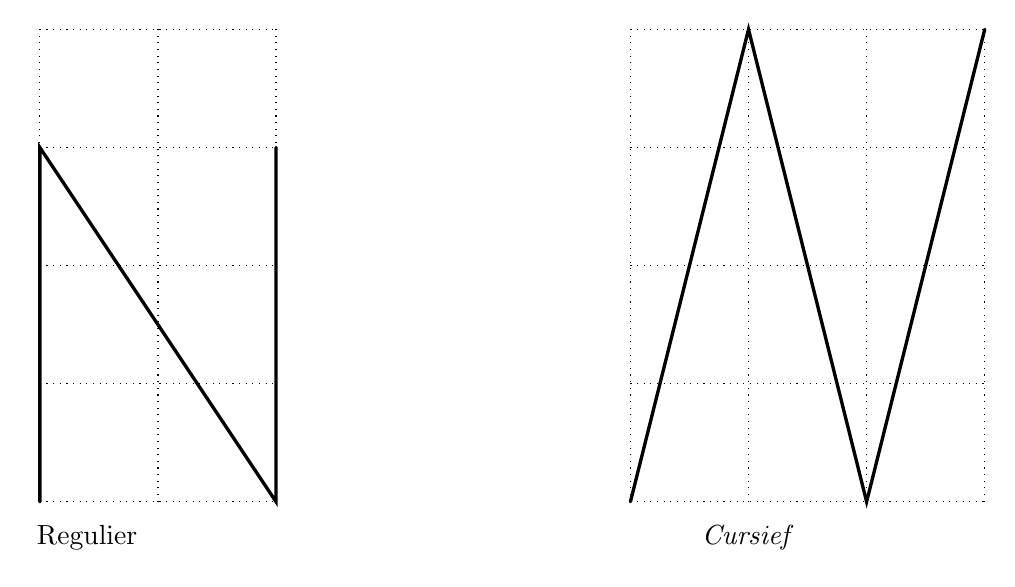
\begin{tikzpicture}[scale=1.5]
\begin{scope}
\draw[step=1, dotted] (0,0) grid (2,4);
\draw[very thick, line cap=round] (0,0) -- (0,3) -- (2,0) -- (2,3);
\node at (0.4,-0.3) {Regulier};
\end{scope}

\begin{scope}[xshift=5cm]
\draw[step=1, dotted] (0,0) grid (3,4);
\draw[very thick, line cap=round] (0,0) -- (1,4) -- (2,0) -- (3,4);
\node at (1,-0.3) {\textit{Cursief}};
\end{scope}
\end{tikzpicture}
\end{figure}

\subsection*{Open problemen}

\begin{exercise}
    Vind een matrix $A$ die de ``N'' transformeert van een gewoon lettertype van 12-punt groot naar een cursief lettertype van 16-punt groot.
    Schrijf jullie oplossing en aanpak uit, en maak een lijst van eventuele aannames die jullie maken, of eventuele vragen voor verdere uitwerking die bij jullie opkomen.
    \begin{hint}
    Als we co oordinaten toekennen aan de hoekpunten van de kleinere ``N'', krijgen we de volgende punten:
    \[\begin{pmatrix}0 \\ 0\end{pmatrix}, \begin{pmatrix}0 \\ 3\end{pmatrix}, \begin{pmatrix}2 \\ 0\end{pmatrix}, \begin{pmatrix}2 \\ 3\end{pmatrix}\]
    Wat moeten de coordinaten zijn na de transformatie?
    \end{hint}
\end{exercise}

\begin{exercise}
Vorig semester beschreven twee andere leerlingen de volgende aanpak.
Lees hun beschrijving hieronder.

\begin{quote}
\textit{``Om de matrix $A$ te vinden, gaan we een matrix vinden die de langere ``N'' maakt (verticaal uitrekken), een matrix vinden die de kortere ``N'' schuintrekt, en dan het product van die twee vinden om de gewenste matrix $A$ te krijgen.''}
\end{quote}

Denk je dat deze aanpak werkte om matrix $A$ te vinden?
Lijkt het verstandig?
Zoja, denk je dat het dezelfde matrix $A$ is die we in het vorige probleem vonden?
\end{exercise}

\begin{exercise}
Probeer de voorgestelde aanpak. Je moet ofwel:
\begin{enumerate}
\item[(a)] Een matrix $A$ vinden door hun aanpak te gebruiken, of
\item[(b)] Expliciet uitleggen waarom deze aanpak niet werkt.
\end{enumerate}
\begin{oplossing}
    De aanpak werkt wel degelijk. We kunnen de volgende stappen volgen:
    \begin{enumerate}
        \item We rekken alle \(y\)-coördinaten uit met een factor \(\frac{4}{3}\), maar laten de \(x\)-coördinaten ongewijzigd. Dit geeft ons de matrix:
        \[S = \begin{bmatrix} 1 & 0 \\ 0 & \frac{4}{3} \end{bmatrix}\]
        \item Vervolgens moeten we de figuur schuintrekken om het cursieve effect te bereiken.
        Punten op de \(x\)-as blijven onveranderd, terwijl punten hogerop meer naar rechts worden verschoven.
        Bijvoorbeeld, het punt \((2, 4)\) moet naar \((3, 4)\) worden getransformeerd.
        Als we zouden inzoomen op de ``N'', dan zou bijvoorbeeld het punt \((20,40)\) getransformeerd moeten worden naar \((30,40)\).
        We willen met andere woorden een verschuiving toevoegen van \(1\) eenheid in de \(x\)-richting voor elke \(4\) eenheden dat het punt in de \(y\)-richting ligt.
        Dit geeft ons de schuintrekmatrix:
        \[H = \begin{bmatrix} 1 & \frac{1}{4} \\ 0 & 1 \end{bmatrix}\]
        \item De totale transformatie is dan het product van deze twee matrices:
        \[A = H \cdot S = \begin{bmatrix} 1 & \frac{1}{4} \\ 0 & 1 \end{bmatrix} \cdot \begin{bmatrix} 1 & 0 \\ 0 & \frac{4}{3} \end{bmatrix} = \begin{bmatrix} 1 & \frac{1}{3} \\ 0 & \frac{4}{3} \end{bmatrix}\]
    \end{enumerate}
    Is het belangrijk in welke volgorde we de transformaties toepassen, of met andere woorden welke matrix we eerst vermenigvuldigen?
\end{exercise}

\begin{exercise}
    Stel dat we een andere letter zoals een ``A'' willen omzetten naar het cursief lettertype van 16-punt groot, startend vanaf het reguliere lettertype van 12-punt groot.
    Mogen we dan dezelfde matrix $A$ gebruiken als in de vorige oefeningen?
    Of moeten we een andere matrix vinden voor elke letter?
    \begin{figure}[H]
    \begin{tikzpicture}[scale=1.5]
    \begin{scope}
    \draw[step=1, dotted] (0,0) grid (2,4);
    \draw[very thick, line cap=round] (0,0) -- (1,3) -- (2,0);
    \draw[very thick, line cap=round] (0.5,1.5) -- (1.5,1.5);
    \node at (0.4,-0.3) {Regulier};
    \end{scope}

    \begin{scope}[xshift=5cm]
    \draw[step=1, dotted] (0,0) grid (3,4);
    \draw[very thick, line cap=round] (0,0) -- (2,4) -- (2,0);
    \draw[very thick, line cap=round] (1,2) -- (2,2);
    \node at (1,-0.3) {\textit{Cursief}};
    \end{scope}
    \end{tikzpicture}
    \end{figure}
    \begin{oplossing}
    Ja, we kunnen dezelfde matrix $A$ gebruiken voor elke letter.
    De matrix $A$ beschrijft een algemene transformatie die alle punten in het vlak aanpast volgens dezelfde regels.
    Het is eigenlijk geen transformatie van individuele punten, maar van volledige deelruimtes.
    (In een volledig realistisch scenario zou de matrix ook rekening moeten houden met de specifieke kenmerken van elke letter, maar in dit vereenvoudigde voorbeeld is dat niet nodig.)
    \end{oplossing}
\end{exercise}
\end{document}